% !TEX encoding = MacOSRoman
\documentclass{beamer}
\usepackage[utf8]{inputenc}
\usepackage{amsfonts}
\usepackage{textcomp}
\usepackage{listings}
\usepackage{graphicx}
\usepackage{numprint}
\usepackage{subfigure}
\usepackage{tikz}
\usetikzlibrary{shapes.geometric, arrows}
\usepackage{setspace}
%\usepackage{termlist}
\usepackage{amsmath}
\usepackage{amsmath}
\usepackage{amssymb}
\usepackage{amsthm}
\usepackage{bm} 
\usetikzlibrary{arrows,automata}
\usepackage{pgf}
 
\newcommand{\samelineand}{\qquad} 
 
%Information to be included in the title page:
\title{Analysis of time delay data and clock drift in a network of seismic monitors}
\author{Jordi Anguera \inst{1} \and 
Leevi Annala \inst{2} \and 
Stefan Dimitrijevic \inst{3} \and 
Patricia Pauli \inst{4} \and 
Liisa-Ida Sorsa \inst{5} \and 
Dimitar Trendafilov \inst{6} \and 
Christophe Pickard \inst{7}}

\institute[XLIM]{\inst{1} Autonomous University of Barcelona, Spain \samelineand 
	\inst{2}University of Jyvaskyla, Finland \and 
	\inst{3} University of Novi Sad, Serbia \samelineand 
	\inst{4}Technical University of Darmstadt, Germany \and 
	\inst{5}Tampere University of Technology, Finland  \and 
	\inst{6} University of Sofia ''St. Kliment Ohridski'', Bulgaria \and 
	\inst{7} University of Grenoble Alpes and Grenoble INP, France}
\date{ECMI Modelling Week, 21 July 2018} 
 
\begin{document}
 
\frame{\titlepage}

\makeatletter
\makeatother

\section{Problem statement}
\begin{frame}
\frametitle{Problem statement}
\begin{itemize}
\item Seismic monitoring is used to study the behaviour and composition of the underground floor
\item There is a time drift in the monitors' clocks, causing inaccuracies in analysis
\item Continuous synchronisation to the Global Positioning System for accurate timing is not possible 
\item A reliable method to correct the time drift of the clocks' is required
\end{itemize}
\end{frame}

\section{Data}

\begin{frame}
\frametitle{The network of seismic monitors}
\begin{itemize}
\item The network consists of 73 seismic monitors
\item For initial analysis, 7 stations are selected
\end{itemize}

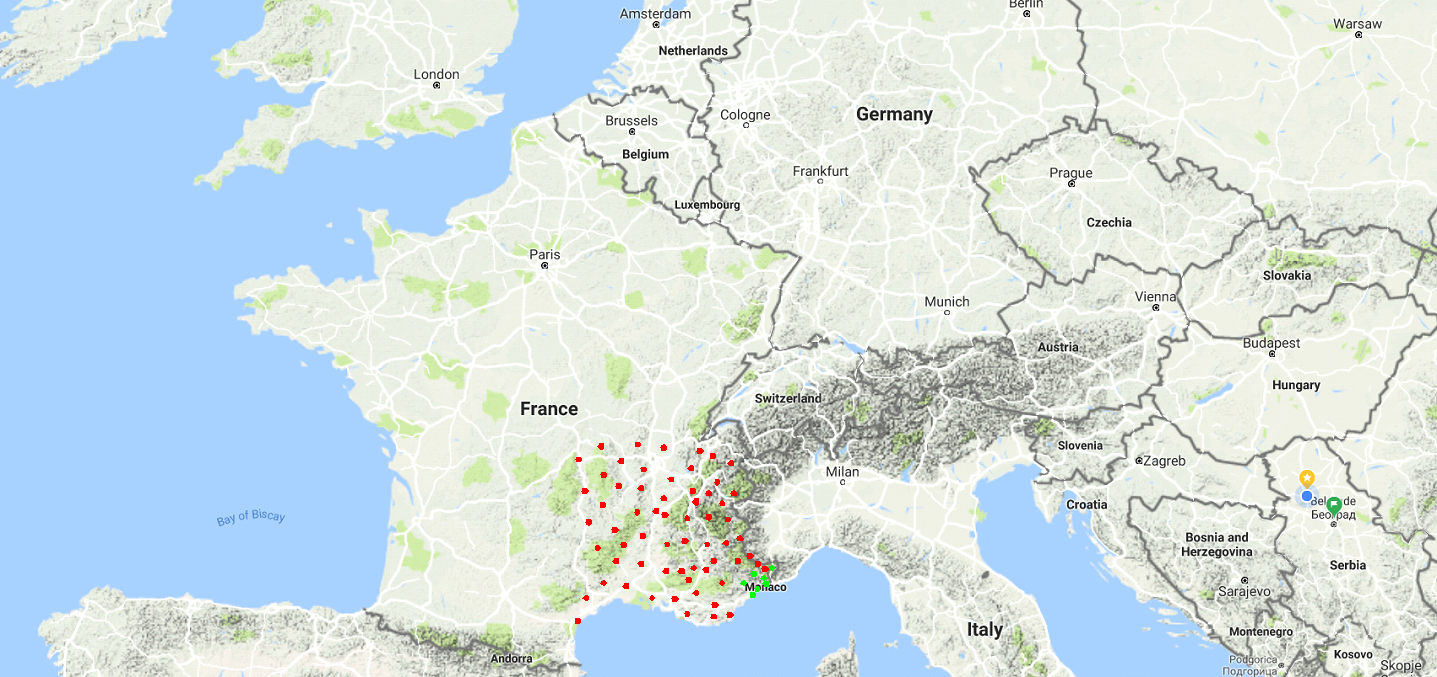
\includegraphics[width=\textwidth]{InitialStationSet.png}
\end{frame}

\begin{frame}
\frametitle{The network of seismic monitors}
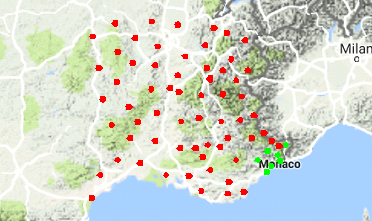
\includegraphics[width=\textwidth]{InitialStationSet_zoom.png}
\end{frame}

\begin{frame}
\frametitle{Numbers of working stations and connections of stations during one year}
\begin{itemize}
\item The maximum of simultaneously working stations is 52 out of 73
\item The maximum of connections is 1326
\item If two monitors are working simultaneously, they are connected
\end{itemize}

\begin{columns}
\column{0.5\textwidth}
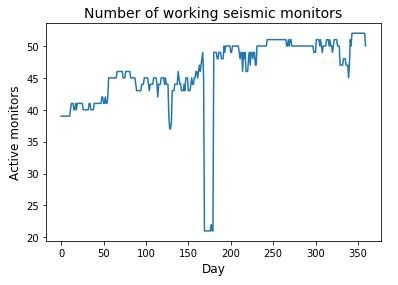
\includegraphics[width=\textwidth]{working_monitors-presentation.png}

\column{0.5\textwidth}
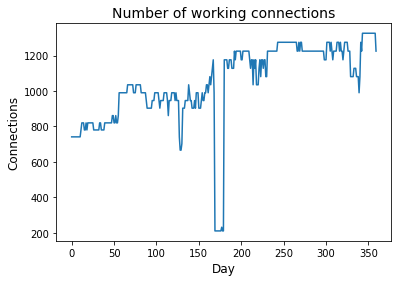
\includegraphics[width=\textwidth]{working_connections_presentation.png}
\end{columns}
\end{frame}

\begin{frame}
\frametitle{Time-delay signal characteristics}
\begin{itemize}
\item Data recorded in one second intervals
\item Time-delay cross-correlation is computed in one-hour intervals
%\item Each connection is computed only once 
\item Recording time is one year
\end{itemize}

\begin{columns}
\column{0.5\textwidth}
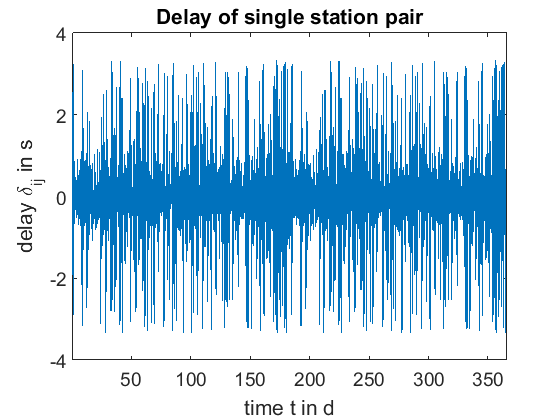
\includegraphics[width=\textwidth]{delayevolutionovertimeforonestation2_presentation.png}

\column{0.5\textwidth}
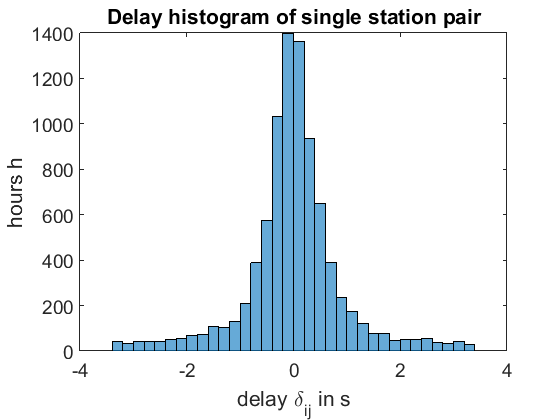
\includegraphics[width=\textwidth]{delayevolutionovertimeforonestation_presentation.png}
\end{columns}
\end{frame}

\begin{frame}
\frametitle{Histograms showing time delays recorded by all active stations over 24 hours}
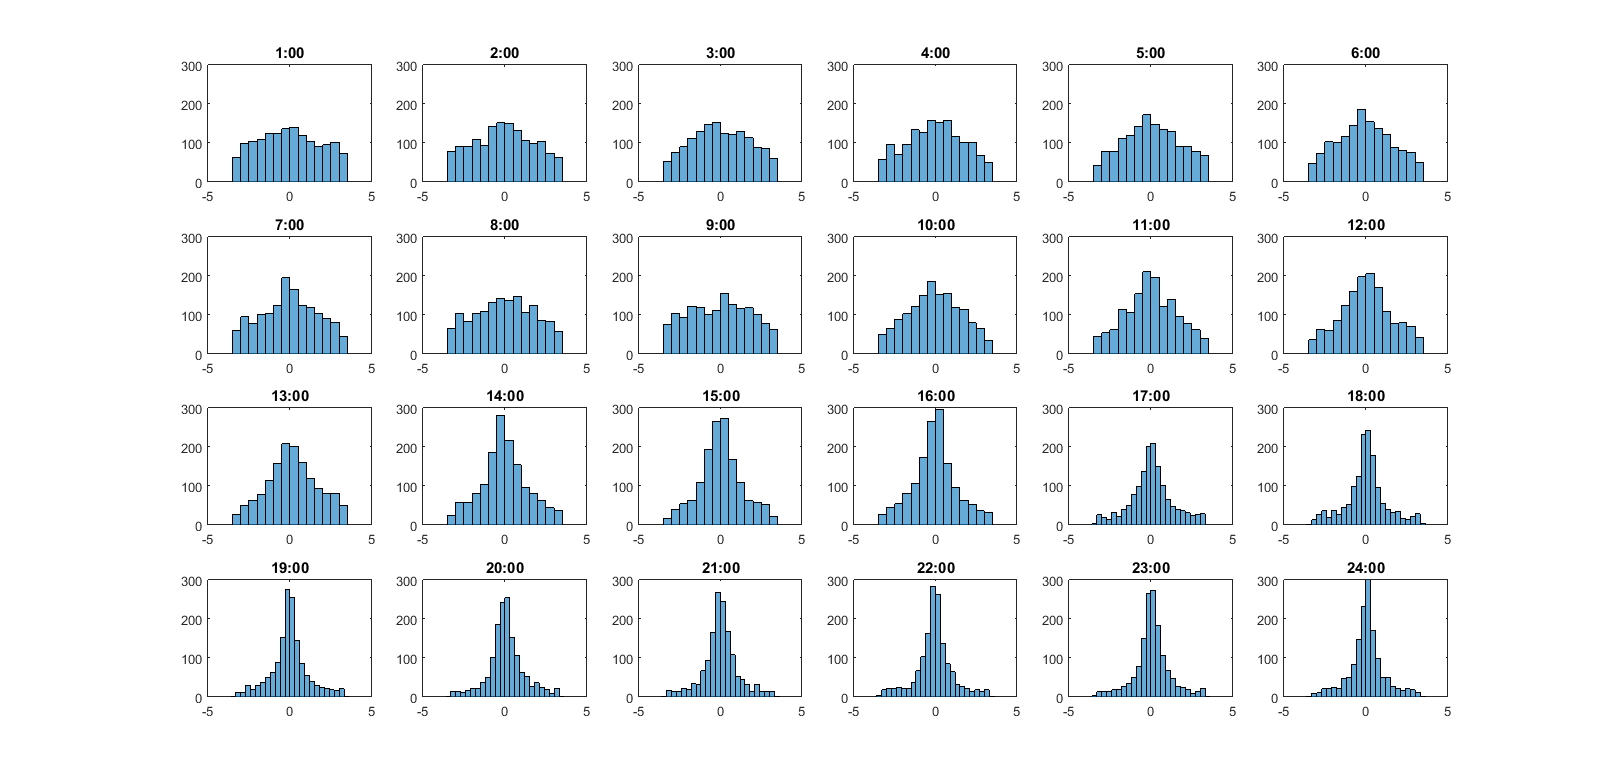
\includegraphics[width=\textwidth]{hourlydelaydistributionoverallstationsforoneday.png}
\end{frame}

\begin{frame}
\frametitle{Comparison of time delay of the furthest and the closest station pairs}
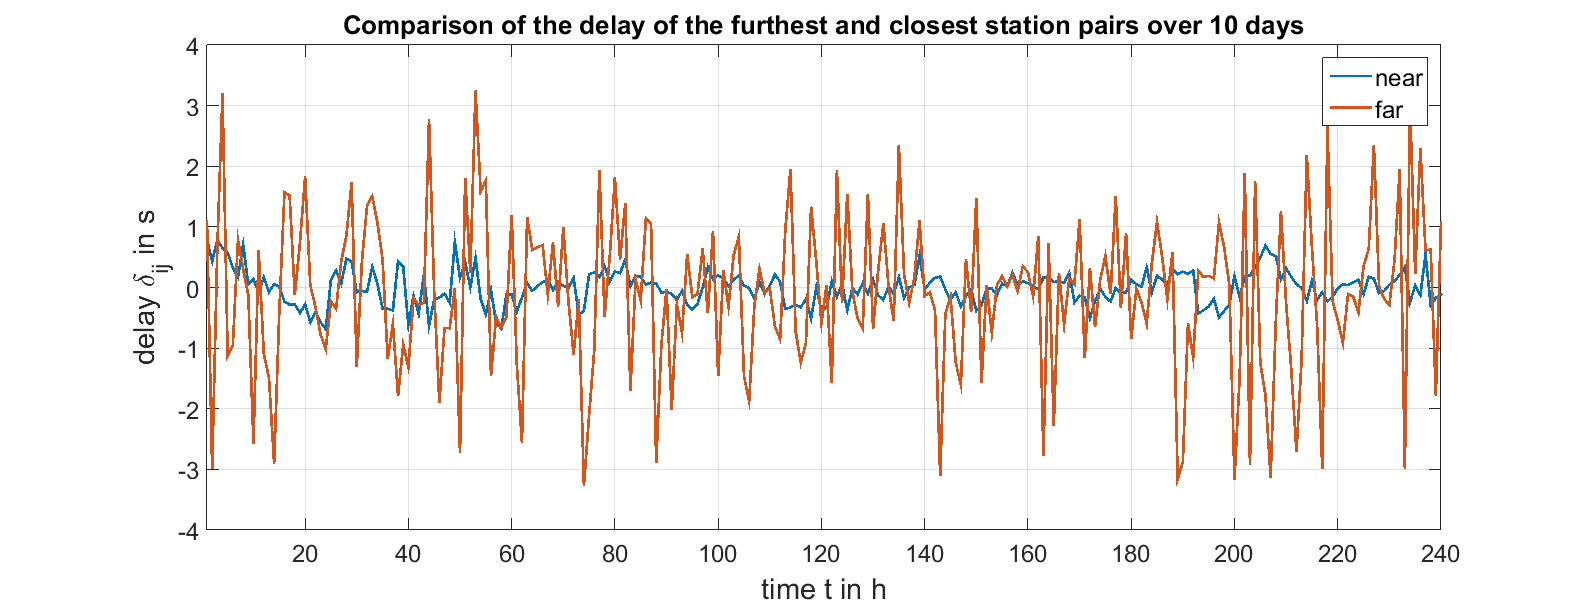
\includegraphics[width=\textwidth]{Comparisondelayoverrandomdayoffarestandclosestlinks_presentation.png}

\begin{itemize}
\item Time delays are smaller between stations which are close to each other
\end{itemize}
\end{frame}

\section{Model}

\begin{frame}
\frametitle{Graph approach to model the data}
\begin{itemize}
\item Measured time delays $\bm{\hat{\delta}}$ between stations:
\begin{equation}
\bm{\hat{\delta}}  = \bm{\delta}(t) + \bm{\varepsilon}(t)
\label{eq:model}
\end{equation}

\item Graphs $\mathcal{G}_{\delta} = (\mathcal{V}, \mathcal{E}, \bm{\hat{\delta}})$, $\mathcal{G}_r = (\mathcal{V}, \mathcal{E}, \bm{W})$

\item Metric:
\begin{equation}
f_i(\bm{\hat{\delta}})=K_i
\end{equation}
with
\begin{equation}
f_i(\bm{\hat{\delta}})=\sum_j\delta_{ij} \quad \text{and} \quad K_i = f_i (\bm{W})= \sum_j{w_{ij}}  
\end{equation}

\end{itemize}

\begin{columns}
\column{0.3\textwidth}
\resizebox{\textwidth}{!}{
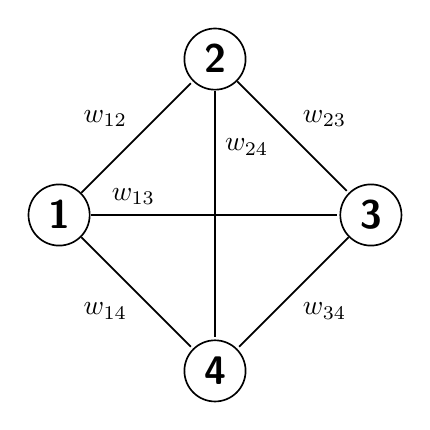
\begin{tikzpicture}[main node/.style={circle,draw,font=\sffamily\Large\bfseries},>=stealth',shorten >=1pt,auto,node distance=2.8cm,
                    semithick]
  \tikzstyle{every state}=[draw=none]

  \node[main node] (1) {1};
  \node[main node] (2) [above right of=1] {2};
  \node[main node] (4) [below right of=1] {4};
  \node[main node] (3) [below right of=2] {3};

  \path (1) edge node {$w_{12}$} (2)
            edge node [above left, pos=0.3] {$w_{13}$} (3)
            edge node [below left] {$w_{14}$} (4)
        (2) edge node {$w_{23}$} (3)
       		 edge node [above right, pos=0.3] {$w_{24}$} (4)
        (3) edge node {$w_{34}$} (4);
\end{tikzpicture}
}
\column{0.3\textwidth}
\resizebox{\textwidth}{!}{
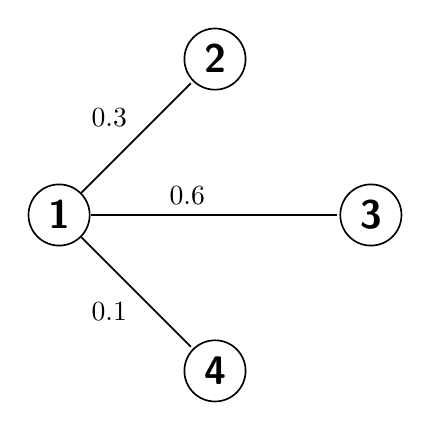
\begin{tikzpicture}[main node/.style={circle,draw,font=\sffamily\Large\bfseries},>=stealth',shorten >=1pt,auto,node distance=2.8cm,
                    semithick]
  \tikzstyle{every state}=[draw=none]

  \node[main node] (1) {1};
  \node[main node] (2) [above right of=1] {2};
  \node[main node] (4) [below right of=1] {4};
  \node[main node] (3) [below right of=2] {3};

  \path (1) edge node {$0.3$} (2)
            edge node [above left] {$0.6$} (3)
            edge node [below left] {$0.1$} (4);
\end{tikzpicture}
}
\column{0.3\textwidth}
text here
\end{columns}

\end{frame}

\begin{frame}
\frametitle{Signal denoising and exctracting clock drift}
\begin{itemize}
\item We specify a cost function $c(\bm{\hat{\delta}})$ measuring the deviation of the metric:
\begin{equation}
c(\bm{\hat{\delta}}) = \sum_i e_i^2(\bm{\hat{\delta}}) = \sum_i(f_i(\bm{\hat{\delta}})-K_i)^2
\end{equation}

\item Error is minimized with gradient descent updates on $\bm{\hat{\delta}}$: 

\begin{equation}
\bm{\hat{\delta}}^{(t+1)} = \bm{\hat{\delta}}^t-\mu\sum_i e_i(\bm{\hat{\delta}}^t)\frac{df_i(\bm{\hat{\delta}}^t)}{d\bm{\hat{\delta}}^t}
\label{eq:updates}
\end{equation}

\item The noise $\varepsilon_{ij}$ between each pair of two stations is caused by clock drifts $\Delta_i$ and $\Delta_j$, and other errors $e_{ij}$:
\end{itemize}
\begin{equation}
\varepsilon_{ij} = \Delta_i - \Delta_j + e_{ij}
\end{equation}

\end{frame}

\begin{frame}%[shrink=20]
\frametitle{Solving individual clock drifts (1/2)}
\begin{itemize}
\item We have overdetermined inverse problem of the form
\begin{equation}
\bm{Gs} = \bm{m}
\end{equation}

\footnotesize
\begin{equation*}
\begin{bmatrix}
1 & -1 & 0 & 0 & \dots  & 0 \\
1 & 0 & -1 & 0 & \dots  & 0 \\
1 &  0  & 0 & -1 & \dots   & 0 \\
\vdots & \vdots & \vdots  & \vdots & \ddots & \vdots \\
1 &  0  & 0 & 0 & \dots & -1 \\
0 &  1  & -1 & 0 & \dots & 0 \\
0 & 1 & 0 & -1 & \dots & 0 \\
0 & 1 & 0 & 0 & \ddots & 0 \\
\hdotsfor{6} \\
0 & 0 & \dots & 0& 1 & -1
\end{bmatrix}
 \begin{bmatrix}
\Delta_1 \\ \Delta_2 \\ \Delta_3 \\ \Delta_4 \\ \vdots \\ \Delta_k \\ \vdots \\ \Delta_{n-1} \\ \Delta_n
\end{bmatrix}
 = 
 \begin{bmatrix}
 \Delta_1 - \Delta_2 \\ \Delta_1-\Delta_3 \\ \Delta_1-\Delta_4 \\ \vdots \\ \Delta_1 - \Delta_{n} \\ \Delta_2- \Delta_3 \\ \Delta_2 - \Delta_4 \\ \vdots  \\ \Delta_2-\Delta_k \\ \vdots \\ \Delta_{n-1} - \Delta_n
 \end{bmatrix}
= 
\begin{bmatrix}
\Delta_{12} \\ \Delta_{13} \\ \Delta_{14} \\ \vdots \\ \Delta_{1n} \\ \Delta_{23} \\ \Delta_{24} \\ \vdots \\ \Delta_{2k} \\ \vdots \\ \Delta_{(n-1)n}
\end{bmatrix} 
\end{equation*}
\normalsize

\item Matrix $\bm{G}$'s rank is $n-1$
\end{itemize}
\end{frame}

\begin{frame}
\frametitle{Solving individual clock drifts (2/2)}
\begin{itemize}
\item Ordinary least squares regression
\begin{equation}
\| \mathbf{Gs}-\mathbf{m} \|_2^2.
\label{eq:leastsquares}
\end{equation}

\item Tikhonov regularization is employed
\begin{equation}
\| \mathbf{Gs}-\mathbf{m} \|_2^2 + \| \bm{\Gamma}\mathbf{s} \|_2^2, 
\label{eq:tikhonov}
\end{equation}
\quad \quad for some suitable Tikhonov matrix $\bm{\Gamma} = \alpha\mathbf{I}$
\item The explicit solution is hence given by
\begin{equation}
\hat{\mathbf{s}} = (\mathbf{G}^T\mathbf{G} + \bm{\Gamma}^T\bm{\Gamma})^{-1}\mathbf{G}^T\mathbf{m}.  
\end{equation}

\end{itemize}

\end{frame}

\section{Results}
\begin{frame}
\frametitle{Signal - denoised signal - noise}
\begin{columns}
\column{0.3\textwidth}
Full signal from one connection for 10 hours

\vspace{1.8cm}

Denoised signal of the connection

\vspace{1.8cm}

Signal noise

\column{0.6\textwidth}
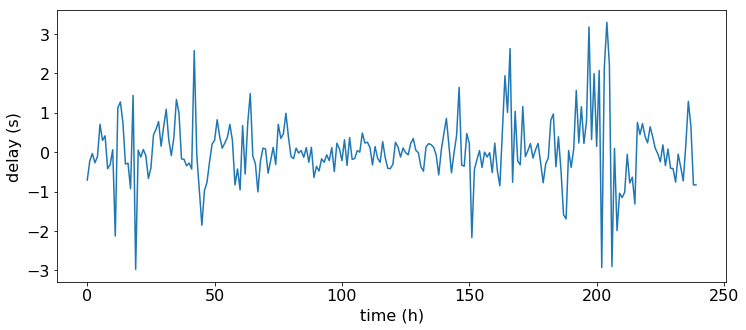
\includegraphics[height=0.28\textheight]{noisy-time-delay-data-10-days.png}

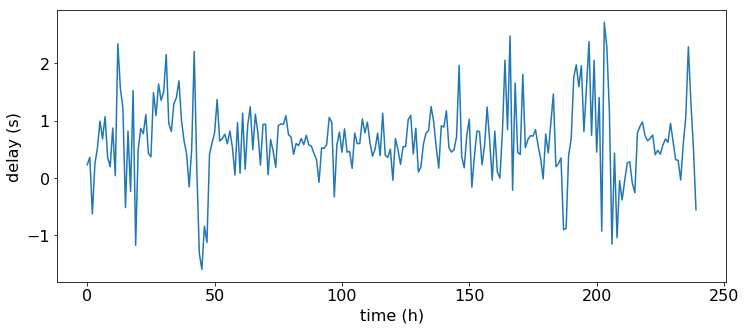
\includegraphics[height=0.28\textheight]{denoised-time-delay-data-ten-days.png}

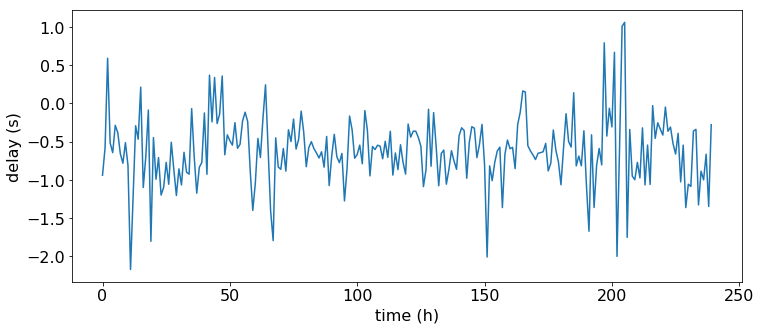
\includegraphics[height=0.28\textheight]{the-noise-ten-days.png}

\end{columns}

\end{frame}

 \begin{frame}
\frametitle{Clock drifts}
Figure here
\end{frame}

\section{Conclusion}
 \begin{frame}
\frametitle{Conclusion}
\begin{itemize}
\item A graph method to recover clock drift in large time-delay network was developed
\item Clock drifts for the three most influential monitors and five others close by were computed
\item Clock drift may account for up to 1 \% inaccuracy in timing at each time point
\item The drift varies over time
\end{itemize}
\vspace{0.5cm}
\textbf{\large{Future work:}}\normalsize 
\begin{itemize}
\item A synthetic dataset to verify the effectiveness of the method
\item Analyze the complete network of monitors
\item Develop and test other metrics
\item Carry out sensitivity analysis
\end{itemize}
\end{frame}

\end{document}

